\section{Aufgabe 29 "Die Likelihoodkurve"}

\begin{figure}[ht]
   \centering
 \includegraphics[width=0.9002\textwidth]{aufg29.jpg}
   \label{fig1}
\end{figure}


\begin{figure}
    \includegraphics{/home/hubi/smd1718/Blatt10/output/aufg29.pdf}
    \label{}
\end{figure}

\section{Aufgabe 30 " F- Praktikum"}
a.) Berechung der Design Matrix
$$
\underline{ \underline{A}}=
\begin{pmatrix}
    \cos(0) &\sin(0) \\
    \cos(30) &\sin(30) \\
    \cos(60) &\sin(60) \\
    \cos(90) &\sin(90) \\
    \cos(120) &\sin(120) \\
    \cos(150) &\sin(150) \\
    \cos(180) &\sin(180) \\
    \cos(210) &\sin(210) \\
    \cos(240) &\sin(240) \\
    \cos(270) &\sin(270) \\
    \cos(300) &\sin(300) \\
    \cos(330) &\sin(330) \\
\end{pmatrix}
=
\begin{pmatrix}
   1 &  0    \\
  0.866 &  0.5   \\
  0.5  & 0.866   \\
  0  & 1   \\
 -0.5  & 0.866   \\
 -0.866  & 0.5   \\
 -1  & 0   \\
 -0.866  &-0.5   \\
 -0.5  &-0.866   \\
 0  &-1   \\
  0.5  &-0.866   \\
  0.866  &-0.5   \\
\end{pmatrix}
$$
b.)
Der Lösungsvektor berechnet sich wie folgt:
$$
\hat{a}=(\text{A}^\text{T}\text{A})^{-1}\text{A}^\text{T}\vec{y}
$$
Die Berechnung wurde in der main.py durchgeführt.
Es ergibt sich somit für dien Lösungsvektor: $ a=(-0.0375, 0.0774)^\text{T}$\\
c.)\\
Die Berechnung der Kovarianzmatrix erfolgt ebenfalls in der main.py, diese
berechnet sich wie folgt:
$$
\text{V}[\hat{a}]=(\text{A}^\text{T}\text{A})^{-1}\text{A}^\text{T}=
\begin{pmatrix}
6.84 & -4.74 \\
-5.42 & 6.84 \\
\end{pmatrix}
$$
Für die Fehler ergibt sich :
$$\begin{pmatrix}
a_1 \\
a_2 \\
\end{pmatrix}
=
\begin{pmatrix}
0.261 \\
0.261
\end{pmatrix}
$$
d.)\\
Für die Koeffizienten aus der Theorie folgt:
$$A_0=-0.038 \pm 0.026 \quad \quad \quad \delta= 0.077 \pm 0.026 $$


\section{Aufgabe 31 "Regularisierung kleinste Quadrate"}

a.)
\begin{figure}[ht]
   \centering
 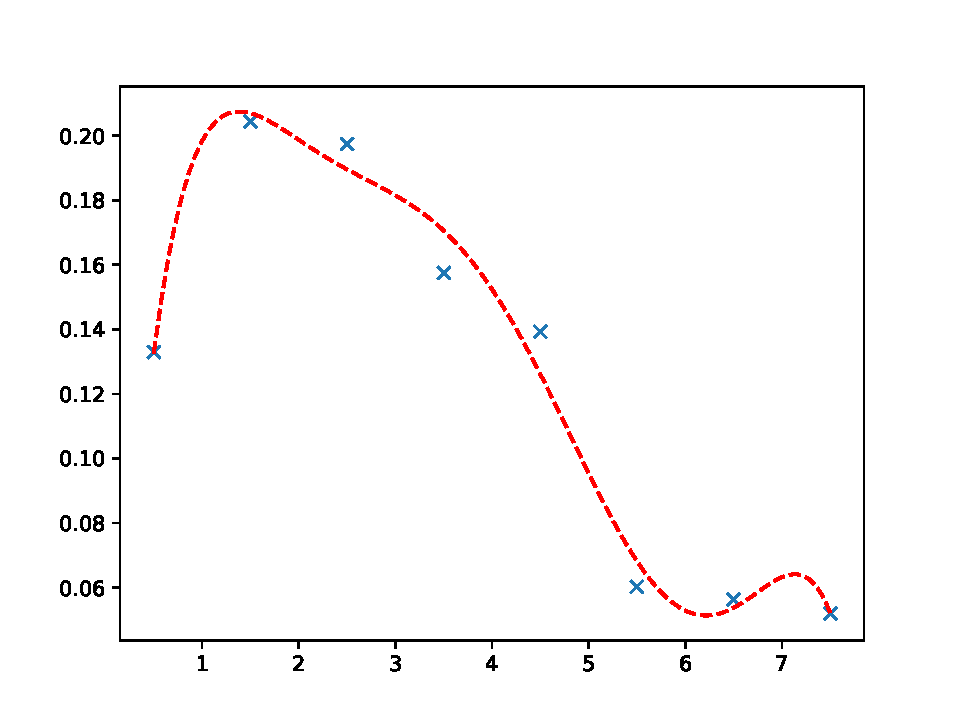
\includegraphics[width=0.82\textwidth]{../output/linreg_sk.pdf}
   \label{fig1}
\end{figure}
b.)
\begin{figure}[ht]
   \centering
 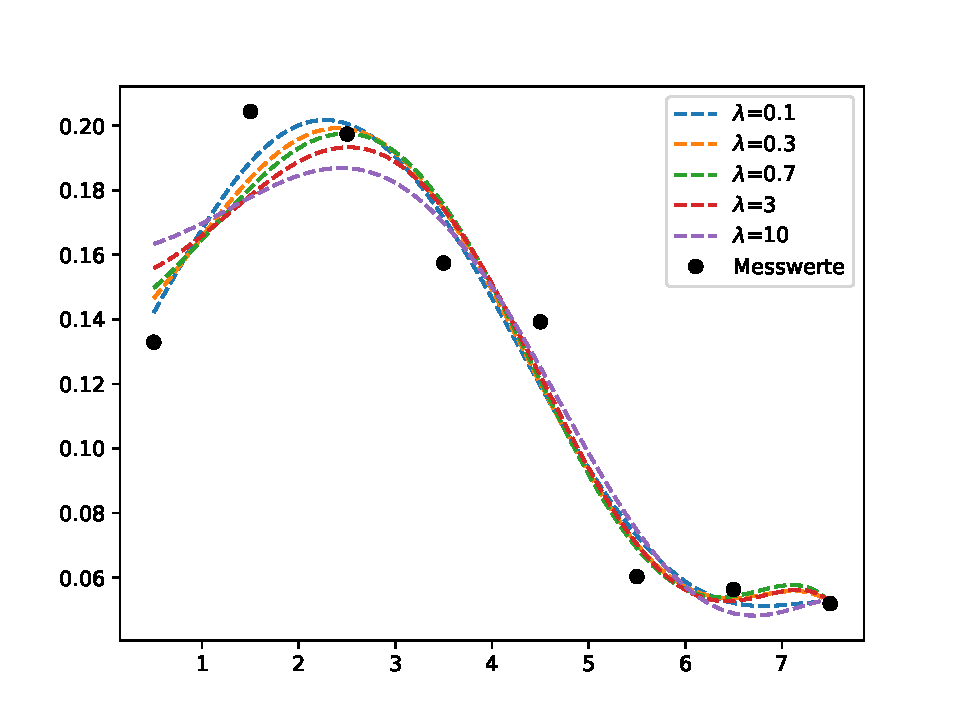
\includegraphics[width=0.82\textwidth]{../output/linreg_sk_ridge.pdf}
   \label{fig1}
\end{figure}
